\scanpage{74}
\mspage{36}
On a comme spécialisation du cas a)
\figure{\begin{tikzpicture}[x=1cm,y=1cm]
\node at (-1,.1) {$(91)$}; \node at (0,.3) {$\unsure{a'}$)};
\fill (2,.2) circle (1.4pt); \fill (4,.2) circle (1.4pt);
\draw (2,.2)..controls (1.25,1.1) and (.25,.6)..(.6,-.1)..controls (.8,-.65) and (1.6,-.1)..(2,.2);
\draw (2,.2)--(4,.2); \draw (2.1,.35)..controls (2.8,.55) and (3.6,.55)..(3.9,.3);
\foreach \x in {2.2,2.35,...,3.8}{\draw (\x,.37)--(\x+.12,.5);}
\node[above] at (2,.65) {$I_1$};\node[below] at (2,.1) {$g_1$};
\node[above] at (4,.65) {$I_2$};\node[below] at (4,.1) {$g_2$};
\node[anchor=west,align=left] at (5.5,.15) {$\begin{gathered}I_1\amalg I_2=I\\g_1+g_2=g-1\\\text{si }g_2=0\quad\deleted{\unsure{quelconque}}\ \inserted{\text{on a }\operatorname{card}I_2\geq2}\\\deleted{\text{on a }I_1\ne\varnothing\text{ (et }I_2\ne\varnothing\text{)}}\end{gathered}$};
\end{tikzpicture}}
\margin{NB \unsure{OPS} $g_2=1$, $g_1=g-2$ pourvu que $g\geq2$; $(I_1,I_2)$ partition quelc. de $I$.}
On a comme spécialisation du cas b), \deleted{\unsure{si on suppose} $g'$}
\figure{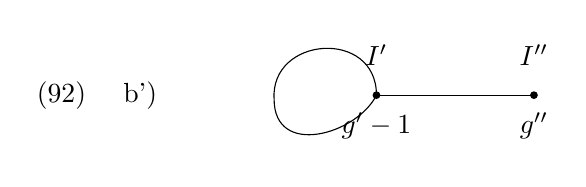
\begin{tikzpicture}[x=1cm,y=1cm]
\node at (-1,0) {$(92)$};\node at (0,0) {b')};
\fill (3,0) circle (1.4pt);\fill (5,0) circle (1.4pt);\draw (3,0)--(5,0);
\draw (3,0)..controls (3,.85) and (1.65,.75)..(1.7,-.05)..controls (1.7,-.8) and (2.75,-.5)..(3,0);
\node[above] at (3,.25) {$I'$};\node[below] at (3,-.1) {$g'-1$};
\node[above] at (5,.25) {$I''$};\node[below] at (5,-.1) {$g''$};
\end{tikzpicture}}
Donc si $g\geq1$ (de sorte que le cas a) existe) alors prenant dans b) \deleted{\unsure{avec} $g'\ne$} les notations $g',g''$ de sorte que $g'\ne0$ i.e. $g'\geq1$ (quitte à éch. $g',g''$), on voit que l'on a une spécialisation \inserted{b') $=$ a')} commune aux cas a) et b). Cela démontre notre assertion lorsque $g\ne0$. \deleted{Si $g$} Dans le cas $g=0$, \inserted{donc $\operatorname{card}I\geq6$}, il n'y a que les cas b), \deleted{et \unsure{OPS}} \deleted{\unsure{a il y a}} Or on a \deleted{\unsure{pour} $\operatorname{card}I'\geq\operatorname{card}I''$, donc $\operatorname{card}I'\geq3$; \unsure{qui a donc} la spécialisation} une spécialisation de la forme
\figure{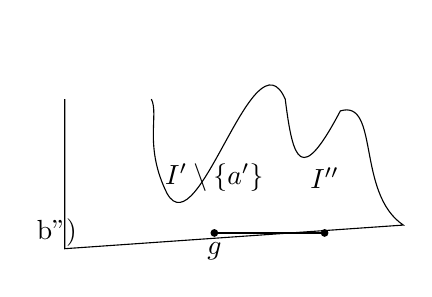
\begin{tikzpicture}[x=1cm,y=1cm]
\node at (0,0) {\deleted{b'')}};
\node at (2,.7) {\deleted{$I'\setminus\{a'\}$}};\node at (3.4,.7) {\deleted{$I''$}};
\fill (2,0) circle (1.4pt);\fill (3.4,0) circle (1.4pt);\draw (2,0)--(3.4,0);
\node[below] at (2,0) {\deleted{$\unsure{g}$}};
\draw (.1,1.7)--(.1,-.2)--(4.4,.1)..controls (3.8,.5) and (4.1,1.7)..(3.6,1.55)..controls (3.1,.6) and (3,0.9)..(2.9,1.7)..controls (2.5,2.6) and (1.8,-.2)..(1.4,.5)..controls (1.1,1.1) and (1.3,1.5)..(1.2,1.7);
\end{tikzpicture}}
\figure{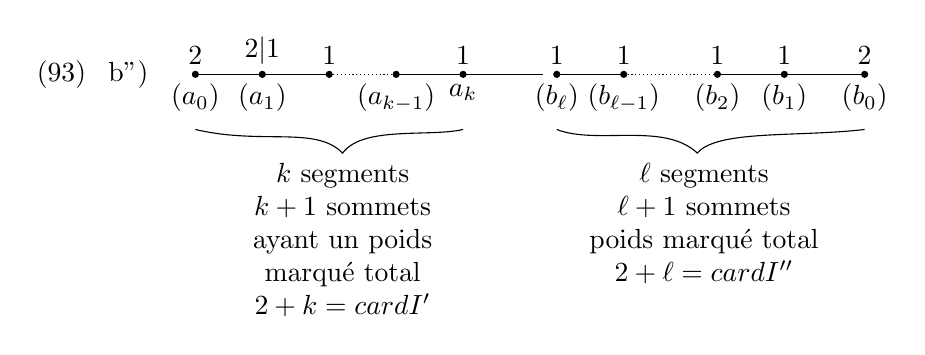
\begin{tikzpicture}[x=.85cm,y=1cm]
\node at (-2,0) {$(93)$}; \node at (-1,0) {b'')};
\draw (0,0)--(2,0) (3,0)--(5.2,0) (5.4,0)--(6.4,0) (7.8,0)--(10,0);
\draw[densely dotted] (2,0)--(3,0) (6.4,0)--(7.8,0);
\foreach \x in {0,1,2,3,4,5.4,6.4,7.8,8.8,10}{\fill (\x,0) circle (1.3pt);}
\node[above] at (0,0) {$2$};\node[below] at (0,0) {$(a_0)$};
\node[above] at (1,0) {$\unsure{2|1}$};\node[below] at (1,0) {$(a_1)$};\node[above] at (2,0) {$1$};
\node[below] at (3,0) {$(a_{k-1})$};\node[above] at (4,0) {$1$};\node[below] at (4,0) {$a_k$};
\node[above] at (5.4,0) {$1$};\node[below] at (5.4,0) {$(b_\ell)$};
\node[above] at (6.4,0) {$1$};\node[below] at (6.4,0) {$(b_{\ell-1})$};
\node[above] at (7.8,0) {$1$};\node[below] at (7.8,0) {$(b_2)$};
\node[above] at (8.8,0) {$1$};\node[below] at (8.8,0) {$(b_1)$};
\node[above] at (10,0) {$2$};\node[below] at (10,0) {$(b_0)$};
\draw (0,-.7)..controls (1,-.9) and (1.8,-.65)..(2.2,-1)..controls (2.5,-.65) and (3.5,-.8)..(4,-.7);
\draw (5.4,-.7)..controls (6,-.9) and (7,-.6)..(7.5,-1)..controls (7.8,-.7) and (9,-.8)..(10,-.7);
\node[anchor=north,align=center] at (2.2,-1) {$k$ segments\\$k+1$ sommets\\ayant un poids\\marqué total\\$2+k=\operatorname{card}I'$};
\node[anchor=north,align=center] at (7.6,-1) {$\ell$ segments\\$\ell+1$ sommets\\poids marqué total\\$2+\ell=\operatorname{card}I''$};
\end{tikzpicture}}
\margin{73}
